\section{Passerelle intelligente}

\begin{frame}{Architecture réseau}
  \begin{figure}
    \centering
    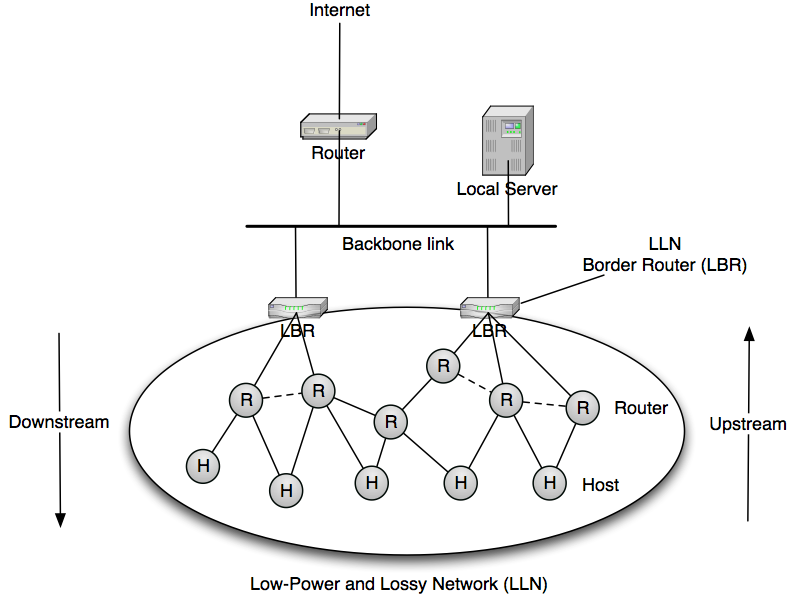
\includegraphics[scale=.3]{figures/rpl.png}
  \end{figure}
\end{frame}

\begin{frame}{Protocoles pour les LLNs}
  \begin{figure}
    \centering
    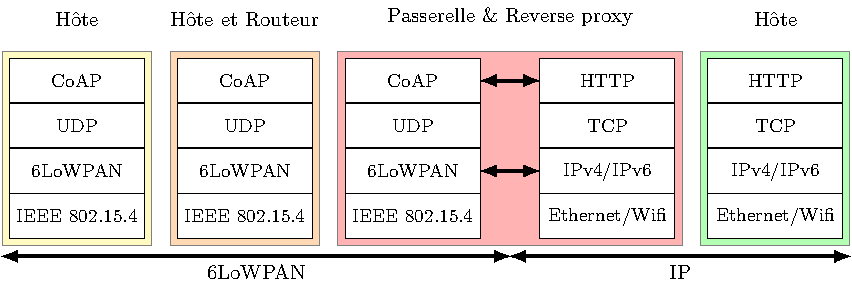
\includegraphics[width=\textwidth]{figures/network_stack_slides.pdf}
  \end{figure}
  
  \pnote{
    - Propos général : les protocoles classiques sont adaptés aux réseaux de capteurs pour en faire des membres à part entières de l'Internet.
  }

  \pnote{
    - IEEE 802.15.4: Couche Physique et MAC; topo maillé/étoilée; Faible cout
  }
  \pnote{
    - 6LoWPAN: Compression IPv6
  }
  \pnote{
    - RPL: Produit les routes montantes et descendantes;
  }
  \pnote{  
    - CoAP: Couche applicative; REST; UDP
  }
\end{frame}

\begin{frame}{Rôle de la passerelle}
  \begin{block}{Couche physique et liaison: \ieee{}}
    \begin{itemize}
      \item PAN coordinator
    \end{itemize}
  \end{block}
  \begin{block}{Couche réseau: 6LoWPAN}
    \begin{itemize}
      \item Compression IPv6
    \end{itemize}
  \end{block}
  \begin{alertblock}{Protocole de routage: RPL}
    \begin{itemize}
      \item Racine du DODAG (MP2P/P2MP)
      \item Routeur de bordure (LBR)
    \end{itemize}
  \end{alertblock}
  \begin{alertblock}{Protocole applicatif: CoAP}
    \begin{itemize}
      \item Traduction de protocole (HTTP/CoAP)
      \item Proxy inverse
    \end{itemize}
  \end{alertblock}
\end{frame}

\begin{frame}{Impact du trafic dans un réseau multi-sauts}
  \begin{figure}
      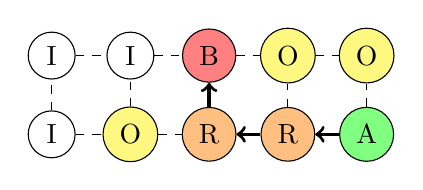
\begin{tikzpicture}
  \tikzstyle{router}=[circle, draw, fill=orange!50,text=black]
  \tikzstyle{child}=[circle, draw, fill=yellow!50,text=black]
  \tikzstyle{root}=[circle, draw, fill=red!50,text=black]
  \tikzstyle{source}=[circle, draw, fill=green!50,text=black]
  \tikzstyle{idle}=[circle, draw, text=black]

  \node[idle] (00) at (0,0) {I};
  \node[child] (10) at (1,0) {O};
  \node[router] (20) at (2,0) {R};
  \node[router] (30) at (3,0) {R};
  \node[source] (40) at (4,0) {A};

  \node[idle] (01) at (0,1) {I};
  \node[idle] (11) at (1,1) {I};
  \node[root] (21) at (2,1) {B};
  \node[child] (31) at (3,1) {O};
  \node[child] (41) at (4,1) {O};

  \path
  % Radio link
  (00.east) edge[dashed] (10.west)
  (10.east) edge[dashed] (20.west)
  (20.east) edge[dashed] (30.west)
  (30.east) edge[dashed] (40.west)

  (01.east) edge[dashed] (11.west)
  (11.east) edge[dashed] (21.west)
  (21.east) edge[dashed] (31.west)
  (31.east) edge[dashed] (41.west)

  (00.north) edge[dashed] (01.south)
  (10.north) edge[dashed] (11.south)
  (20.north) edge[dashed] (21.south)
  (30.north) edge[dashed] (31.south)
  (40.north) edge[dashed] (41.south)

  % Route link
  (40.west) edge[->, very thick] (30.east)
  (30.west) edge[->, very thick] (20.east)
  (20.north) edge[->, very thick] (21.south)
  ;

  \end{tikzpicture}
  \end{figure}
  \begin{block}{Objectifs}
    \begin{itemize}
      \item Calculer l'impact du trafic en fonction de la topologie
      \item Agir de manière aussi transparente que possible
      \item Réguler le trafic si possible
    \end{itemize}
  \end{block}
  \pnote{
    - Certaines requetes ont un plus fort impact que d'autres
  }
  \pnote{
    - Toute les requetes supplémentaires s'additionnent du coup il faut des services aussi transparents que possibles
  }
\end{frame}

\begin{frame}{Reverse proxy}
  \begin{figure}
    \centering
    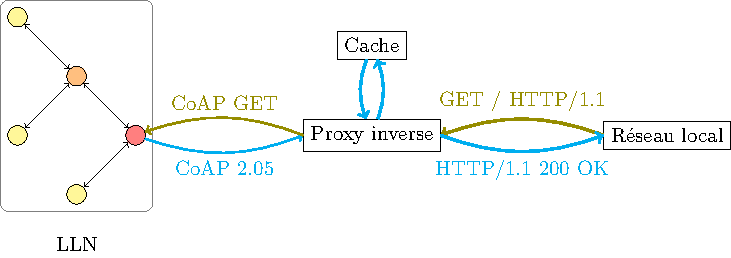
\includegraphics[width=\textwidth]{figures/schema_rpc_slides}
  \end{figure}
  \pnote{
    Reverse proxy: Intermédiaire que l'on contacte et qui va contacter d'autres serveurs.
  }
  \pnote{
    Concept de cache: Invalidation
  }
\end{frame}

\begin{frame}{Problématiques}
  
  \begin{block}{Prévision de l'impact du trafic}
    \begin{itemize}
      \item Provisionnement du réseau
      \item Surveillance matérielle et fonctionnelle continue 
      \item Anticipation des pannes
    \end{itemize}
  \end{block}

  \begin{block}{Optimisation de l'utilisation des ressources}
    \begin{itemize}
      \item Économie de bande-passante et d'énergie
      \item Améliorer la rapidité du traitement
    \end{itemize}
  \end{block}

  \pnote{
    - Avoir une idée de trafic permet de dimensionner son réseau correctement (couverture, routeur intermédiaire)
    Ce qui apporte des gains de fiabilité et aide aux diagnostiques de problèmes.
  }
  \pnote{
    - Suivi de la disponibilité matérielle (un noeud mort) ou fonctionnelle (tout un étage est mort)
  }
  \pnote{
    - Prévoir l'évolution de métriques pour faire des interventions: Niveau de batterie, carte sd saturée
  }
  \pnote{---}
  \pnote{
    - Accorder les demandes des utilisateurs. Les rythmes de requetes importantes.
  }
  \pnote{
    - Servir une réponse depuis la passerelle va plus vite que depuis les noeuds
  }
\end{frame}

% % Annonce des contributions

\begin{frame}\frametitle{Contributions}

  \begin{alertblock}{Supervision passive}
    \begin{itemize}
      \item Observe le trafic au niveau du routeur de bordure
      \item Fournit une estimation de l'utilisation de la radio permettant de déduire une partie de la consommation énergétique
    \end{itemize}
  \end{alertblock}

  \begin{alertblock}{Reverse proxy adaptatif}
    \begin{itemize}
      \item Régule les temps de validité des réponses en cache au niveau de la passerelle
      \item Offre un compromis entre satisfaction des utilisateurs et économies d'énergie
    \end{itemize}
  \end{alertblock}

  \pnote{
    Comment ajouter des services dans le dernier noeud non contraints qui est à la bordure du réseau standard ?
  }
  \pnote{
    - Dire que l'on a d'autres contributions mais que cette présentation se concentre sur celles présentées pour la passerelle.
  }

\end{frame}